% !Mode:: "TeX:UTF-8"
\chapter{深度学习的并行训练}

并行化和分布式计算一直是大规模机器学习中一个让人兴奋的话题, 特别是今天,越来越多的数据被应用到深度神经网络的训练中, 对训练速度提出了很高的要求。
例如,1000h的语音数据的复杂模型(LSTM, BLSTM)训练单卡需要一周左右的时间,而上万小时的数据则需迭代数月才能完成。

而深度学习依赖于大量数据,一般数据量越大,数据覆盖的范围越广,深度学习模型的效果越好。
因此,数据对于深度学习的重要性不言而喻。
海量的训练数据,对深度学习的训练速度提出了更高的要求。
在实际应用中,使用多机多卡(GPU)的解决方案加速深度学习的训练。

主流的深度学习的并行训练大致可以分为两类,基于模型的并行和基于数据的并行。
基于模型的并行,每个Worker分到模型的不同部分,仅负责对局部模型参数的更新,类似Hogwild!\ucite{recht2011hogwild}方法。
数据并行则是将数据分成多份,分别在不同Worker上处理不同的数据,适于大量数据和较小模型的训练方式。

另外一个分类方法是根据模型更新方法可以分为两类,基于梯度的模型更新和直接基于模型的更新。
基于梯度的模型更新,Server的模型更新依赖于梯度计算,如DownpourSGD\ucite{dean2012large}(即DistBelief)和ASGD。
基于模型的更新,Server和Worker的模型更新直接基于模型,通过模型之间的计算更新,如 BSP(Model Average)、EASGD和BMUF等。

本文实现基于MPI(Message Passing Interface) 的BSP、ASGD,EASGD,BMUF四种并行方法。
四种方法均是基于数据并行的方法。
BSP,EASGD和BMUF是基于模型的方法,ASGD是基于梯度的方法。
本章介绍MPI及这四种并行基本原理和实现以及相关实验结果。

\section{MPI并行计算}

MPI是一个标准化的、可移植的消息传递协议。
它由工业界和学术界联合制定,设计了一组可以在异构计算机集群上进行并行计算的接口。
并且,MPI是跨语言的通讯协议,支持多种语言用于编写并行计算机。支持点对点和广播。
MPI协议包括协议和和语义说明,指明其如何在各种实现中发挥其特性。
MPI的目标是高性能,大规模性,和可移植性。MPI在今天仍为高性能计算的主要模型。
MPI有多种实现,例如MPICH,OpenMPI等。

深度学习的并行实现需要在多机多卡之间进行通信。
本文选用MPI作为底层通信协议,本文使用OpenMPI的MPI实现。
本文中使用的MPI的基本接口如表\ref{table:mpi}所示。

%\begin{table}
%    \begin{tabular}{ll}
%    MPI Function    & 作用                 \\
%    MPI\_Init       & MPI初始化             \\
%    MPI\_Comm\_rank & 获取MPI的rank id      \\
%    MPI\_Comm\_size & MPI节点总数            \\
%    MPI\_Allreduce  & MPI所有节点都进行reduce操作 \\
%    MPI\_Send       & MPI发送消息            \\
%    MPI\_Recv       & MPI接收消息            \\
%    \end{tabular}
%\end{table}

\begin{table}[htbp]
	\centering
	\caption{本文使用的MPI的基本接口及其作用}
	\fontsize{10.5pt}{10.5pt}\song \vspace{0.5em}
	\begin{tabularx}{\textwidth}{*2{>{\centering\arraybackslash}X}@{}}
		\toprule
    MPI Function    & 作用                 \\
		\midrule
    MPI\_Init       & MPI初始化             \\
    MPI\_Comm\_rank & 获取MPI的rank id      \\
    MPI\_Comm\_size & MPI节点总数            \\
    MPI\_Allreduce  & MPI所有节点都进行reduce操作 \\
    MPI\_Send       & MPI发送消息            \\
    MPI\_Recv       & MPI接收消息            \\
		\bottomrule
	\end{tabularx}
	\label{table:mpi}
\end{table}




\section{模型平均BSP}

BSP(Bulk Synchronize Parallel),或者称之为模型平均。
其基本思路十分简单,在训练过程中,每隔一段时间对所有Worker上的模型进行同步,
同步的模型是取所有Worker上的模型平均作为更新后的新模型。
假设$w_i$表示同步前每个Worker上的模型,
$\tilde w $表示同步后的模型,$N$为Worker总数。则:
\begin{equation}
\tilde w = \frac{1}{N}\sum\limits_{i = 1}^N {{w_i}}
\end{equation}
基于BSP的并行训练的算法描述如算法\ref{alg:bsp}所示。

\begin{algorithm} \song
\caption{BSP模型平均}
\begin{algorithmic}
\REQUIRE 同步周期$\tau$,学习率$\eta$
%\ENSURE

\textbf{Initial:} $\tilde w$随机初始化,$t_i=0, w_i=\tilde w$,$w_i$表示第$i$个Worker上的模型。
\REPEAT
\FOR{$i\in 1,...,N$,\textbf{parallel}}
\STATE 初始化局部模型$w_i = \tilde w$
\STATE 在$\tau$更新周期内,使用本地数据, 利用SGD更新$w_i$
\STATE ${w_i} = {w_i} - \eta \nabla w_i)$, $\nabla w_i$表示Worker$i$在$t_i$时刻由训练样本的计算梯度。
\ENDFOR
\STATE 更新全局模型: $\tilde w = \frac{1}{N}\sum\limits_{i = 1}^N {{w_i}}$
\STATE ${t_i} = {t_i} + 1$
\UNTIL{(所有样本被处理完)}
\end{algorithmic}
\label{alg:bsp}
\end{algorithm}

基于MPI的BSP算法实现如图\ref{fig:bsp}所示,使用MPI\_Allreduce函数进行Worker间的同步通信。
当到达同步周期时,所有Worker将模型从GPU卡显存复制到CPU的内存中,并除以N,
然后同时调用MPI\_Allreduce函数的SUM操作即可。

\begin{figure}[htbp]
\centering
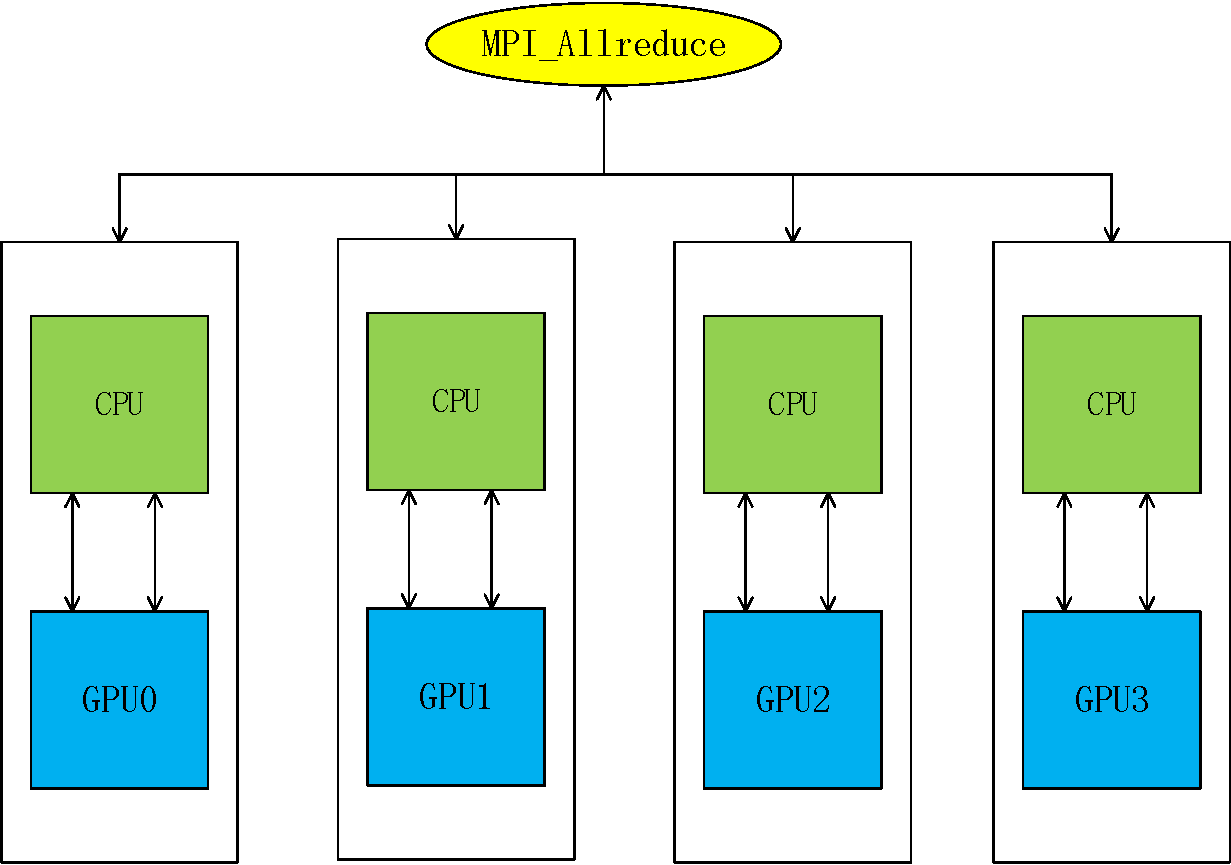
\includegraphics[width=0.5\textwidth]{figures/chapter5/bsp-crop}
\caption{基于MPI的BSP实现}
\label{fig:bsp}
\end{figure}

\section{异步随机梯度下降ASGD}

随机梯度下降SGD(Stochastic Gradient Descent)是深度学习优化的基本原理,
异步随机梯度下降ASGD(Asynchronous SGD)则是随机梯度下降的并行分布式版本。
如图\ref{fig:asgd},ASGD的深度学习系统由两部分组成:
    \begin{enumerate}
        \item 参数服务器Server,负责整体模型的存储和更新。参数服务器Server接收计算节点Worker求得的梯度,
              更新Server上的模型,并把更新后的模型发送给Worker。
        \item $N$个计算节点Worker,Worker根据本地的模型和数据计算出梯度后,将梯度发送给参数服务器,
             并从参数服务器接收最新的模型。
    \end{enumerate}

\begin{figure}[htbp]
\centering
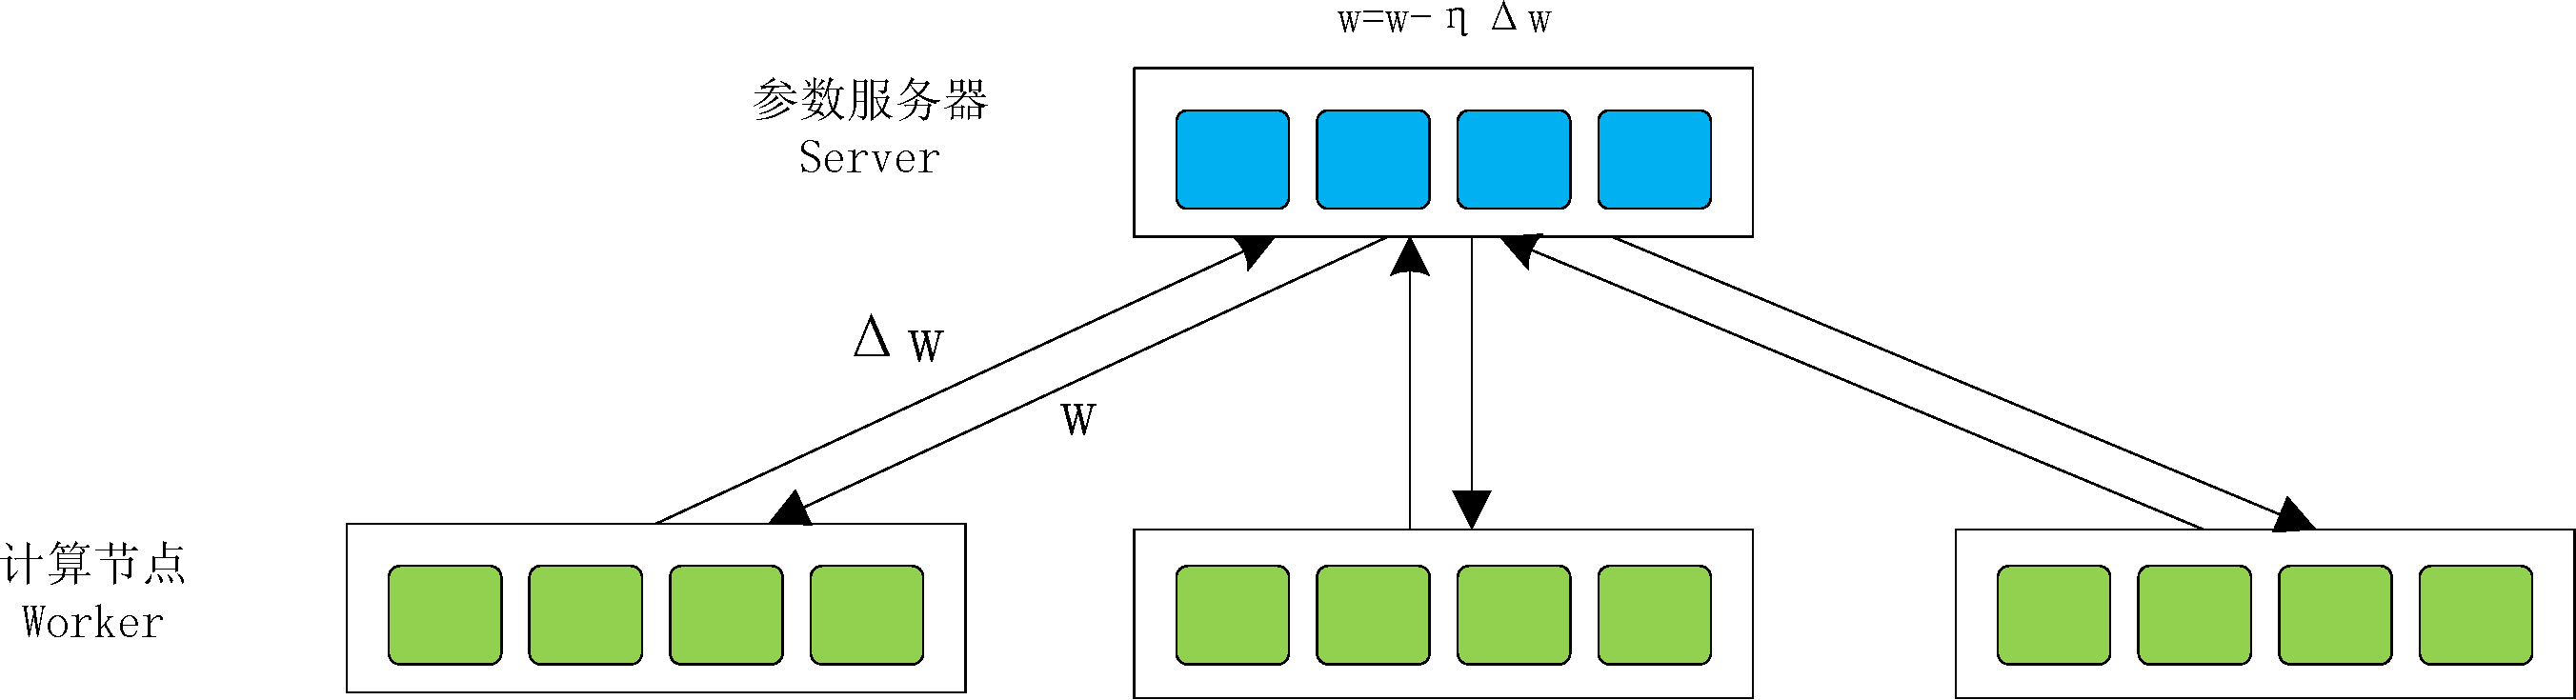
\includegraphics[width=1.0\textwidth]{figures/chapter5/asgd-crop}
\caption{异步梯度下降ASGD}
\label{fig:asgd}
\end{figure}

由图\ref{fig:asgd}可以看出,梯度是在Worker的本地模型上计算得出的梯度,
该梯度最终更新在Server的模型上,计算梯度和梯度更新的并不是同一个模型,所以
称之为异步随机梯度下降。其中Server模型的更新公式为:
\begin{equation}
{\tilde w} = {\tilde w} - \eta \nabla w_i
\end{equation}
其中$\eta$为学习率,$\nabla w_i$为当前Worker上计算发送的梯度。


在ASGD中,各个Worker独立计算,相互之间并不需要通信和同步。
每个Worker均独立和Server进行通信和模型同步,当通信和模型同步频繁时,
Server则会成为系统的性能瓶颈。
在实际应用中,同样会设定一个同步周期$\tau$,Worker计算在该周期内的累加梯度,
然后进行上述更新。$\tau$通过参数调节进行控制,$\tau$越大,Worker更新的频次越低,
系统消耗在模型等待和传输上的时间越少,系统加速的性能越好,但模型的整体效果会越差;
$\tau$越小,更新频次越高,异步程度会降低,模型效果会更好,收敛性更好,
但频繁的模型更新会导致频繁的模型同步,系统的加速性能会下降。
所以,最终同步周期$\tau$的选取则需在模型效果和加速比之间折中。

ASGD中另外一个常用的技巧是设定一个更大的全局同步周期,在该时间节点上时,
将所有Worker和Server上的模型同步为一致。
这样可以防止了各个Worker独立更新导致模型容易发散的问题,
实际应用中,我们发现采用这个技巧后模型的收敛性会更好。

\section{弹性平均随机梯度下降EASGD}

在EASGD\ucite{zhang2015deep}(Elastic Averaging SGD)中,定义优化目标为:
\begin{equation}
\label{equation:easgd}
\mathop {\min }\limits_w F(w) = \sum\limits_{i = 1}^N {f({\rm{S|}}{w_i})} {\rm{ + }}\frac{\lambda }{2}{\rm{||}}{w_i} - \tilde w|{|^2}
\end{equation}
其中$S$代表训练集,$f(.)$代表单卡的神经网络的优化目标,即训练的损失函数,可以是交叉熵CE,最小均方差MSE等的优化准则。
$\lambda$是可调的权重参数,$w_i$表示每个Worker上的模型,$\tilde w $表示Server上的模型。

所以,EASGD的优化目标为使所有Worker上的损失最小,并且各个Worker与Server之间的模型差异也要小, 这样把Worker节点上的参数跟参数服务器的中心变量联系在一起,这样使得Worker本地的模型会围绕中心Server上的模型进行变化。
上面提到,在ASGD中通过设定全局同步周期来防止各个Worker独立计算导致的模型容易发散的问题,
EASGD中则直接通过形式化的方法来达到该目标,$\frac{\lambda }{2}{\rm{||}}{w_i} - \tilde w|{|^2}$类似一个正则项,
强制Worker上的模型围绕Server上的模型进行优化。
$\lambda$比较大时,正则因子越强,Worker的模型倾向于利用当前的Server模型进行优化,
$\lambda$比较小时,正则因子越小,Worker倾向于在当前Server模型的基础上进行更多的探索。

式\ref{equation:easgd}对$\tilde w$和$w_i$进行求导有:
\begin{equation}
\begin{array}{l}
{w_i} = {w_i} - \eta \nabla {w_i} - \eta \lambda ({w_i} - \tilde w)\\
\tilde w = \tilde w - \eta \lambda \sum\limits_{i = 1}^N ( \tilde w - {w_i})
\end{array}
\end{equation}
这是同步的EASGD的更新公式。

在异步的EASGD中,略去Worker自身局部梯度$\nabla {w_i}$,略去同步,令$\alpha  = \eta \lambda$,
则单个Worker对Server模型的更新公式为:
\begin{equation}
\begin{array}{l}
{w_i} = {w_i} - \alpha ({w_i} - \tilde w)\\
\tilde w = \tilde w - \alpha (\tilde w - {w_i})
\end{array}
\end{equation}
$\alpha$控制模型的更新步长。

本文实现并使用异步的EASGD,该算法描述如算法\ref{alg:easgd}所示:
\begin{algorithm} \song
\caption{异步EASGD}
\begin{algorithmic}
\REQUIRE 同步周期$\tau$,学习率$\alpha$ \\
%\ENSURE
\textbf{Initial:} $\tilde w$随机初始化,$t_i=0, w_i=\tilde w$,$w_i$表示第$i$个Worker上的模型。
\REPEAT
\STATE 训练数据样本$s$
\STATE $w=w_i$(中间变量)
\IF{($\tau$整除$t_i$)}
\STATE ${w_i} = {w_i} - \alpha ({w} - \tilde w)$
\STATE $\tilde w = \tilde w - \alpha (\tilde w - {w})$
\ENDIF
\STATE ${w_i} = {w_i} - \eta \nabla w_i(s)$, $\nabla w_i(s)$表示Worker$i$在$t_i$时刻由样本$s$的计算梯度。
\STATE ${t_i} = {t_i} + 1$
\UNTIL{(所有样本被处理完)}
\end{algorithmic}
\label{alg:easgd}
\end{algorithm}

\section{BMUF}

2016年,微软在语音识别任务上提出BMUF\ucite{chen2016scalable}(Block Momentum Update Filtering)并行算法,
并在语音识别任务上取得不错的加速比和更优的模型精度。

BMUF算法同样基于模型。
在训练的一次更新中,首先广播上一时刻的全局模型$\tilde w$到所有Worker,Worker利用$\tilde w$初始化自身模型$w_i$即:
\begin{equation}
w_i = \tilde w
\end{equation}
并在自身的数据上迭代更新$w_i$。

到达同步周期后,需要更新全局模型$\tilde w$。
在BMUF中,使用学习的方法进行更新,即计算梯度,设定学习率,利用梯度方法进行更新。
第$i$个Worker上的梯度为:
\begin{equation}
\nabla {w_i} = {w_i} - \tilde w
\end{equation}
所有Worker上的梯度和为:
\begin{equation}
\nabla {{\tilde w}_t} = \nabla {{\tilde w}_{t - 1}} + \varepsilon \sum\limits_{i = 1}^N {\nabla {w_i}}
\end{equation}
其中$\varepsilon$为冲量Momentum,类似SGD中的冲量。
则全局模型的更新为:
\begin{equation}
\tilde w = \tilde w - \eta \nabla {{\tilde w}_t}
\end{equation}

\begin{algorithm} \song
\caption{BMUF}
\begin{algorithmic}
\REQUIRE 同步周期$\tau$,学习率$\eta$,冲量$\varepsilon$ \\
%\ENSURE

\textbf{Initial:} $\tilde w$随机初始化,$t_i=0, w_i=\tilde w$,$w_i$表示第$i$个Worker上的模型。
\REPEAT
\FOR{$i\in 1,...,N$,\textbf{parallel}}
\STATE 初始化局部模型$w_i = \tilde w$
\STATE 在$\tau$更新周期内,使用本地数据, 利用SGD更新$w_i$
\STATE 计算$\nabla {w_i} = {w_i} - \tilde w$
\ENDFOR
\STATE 收集所有Worker的梯度,并加冲量:
    $\nabla {{\tilde w}_t} = \nabla {{\tilde w}_{t - 1}} + \varepsilon \sum\limits_{i = 1}^N {\nabla {w_i}}$
\STATE 更新全局模型: $\tilde w = \tilde w - \eta \nabla {{\tilde w}_t}$
\UNTIL{(所有样本被处理完)}
\end{algorithmic}
\label{alg:bmuf}
\end{algorithm}

BMUF的算法描述如算法\ref{alg:bmuf}所示。
可以简单比较一下BSP和BMUF。两者在算法的流程上一致,不同之处在于全局模型的更新策略,
BSP中直接取模型平均作为新的模型,而BMUF中则根据梯度进行学习更新,并且引入Momentum加速学习的速率。

同样,简单比较一下EASGD和BMUF。两者在均是基于模型的并行方法,
更新时同样需要计算全局模型和局部模型之间的差分,然后使用该差分更新模型。
不同之处在于:
\begin{enumerate}
\item BMUF是全局同步的方法,每一次更新之后,所有的Worker均使用相同的初始模型;
\item BMUF的差分中引入类似SGD学习中的冲量,而冲量可以加速模型的收敛。
\end{enumerate}

\section{实验}

本文在Kaldi工具包基础上使用OpenMPI实现BSP、ASGD、EASGD、BMUF四种并行方法,
并分别在基于DNN和CLDNN的声学模型上实验验证四种并行训练方法的效果,
分别验证其加速比和相对单卡的模型损失。

\subsection{数据和模型}

类似第四章的实验,本实验同样使用大数据集aslp688,如\ref{data:aslp688}所述。
aslp688共688小时,语料类型为中文普通话朗读数据,共402838句,单句平均时长为6.20s,其中3484句作为交叉验证集,剩余部分全部作为训练集。
测试集同样使用西北工业大学音频语音与语言处理研究组标准测试集test3000,共3063句。

本实验同样使用语音识别工具Kaldi\ucite{povey2011kaldi},深度神经网络使用的对齐由aslp688数据集的GMM-HMM系统产生,共有CD-State状态5389个。
GMM-HMM系统使用39维的MFCC特征,所有深度神经网络均使用40维FBank(Filter Bank)特征。

本节实验中,使用的DNN含7个隐层,使用ReLU作为激活函数,并使用Batch Normalization做相邻层之间的输入归一化,DNN训练中batchsize为256。

使用的CLDNN基本结构中含有1层CNN,2层的DNN和2层的LSTM。
其中CNN中使用40维Fbank特征,不使用差分特征,左右各拼5帧,共440维输入特征,
CNN的卷积层使用128个滤波器,其中滤波器大小为$11 \times 9$,滤波器步移为1,Max Pooling层的步长为4,步移为4,CNN的输出为1024维;
DNN隐层节点为1024;LSTM同样使用LSTMP结构,其中Cell 1024,Projection 512。
CLDNN中的CNN和DNN中使用Sigmoid作为激活函数,同样,CLDNN的相邻层之间使用Batch Normalization做输入归一化。
CLDNN采用跳帧训练,跳帧设置为3帧跳1帧。
CLDNN采用多流训练(即多句话同时训练),每个batch中含有128个流,LSTM的BPTT(Back Propagation Through Time)误差仅往后传20个时刻,所以
batchsize为$128 \times 20 = 2560$。

在DNN和CLDNN的并行训练中,起始训练时均使用单卡第一轮训练的模型作为初始模型,以防止随机初始化造成并行训练难以收敛的问题。

实验所用环境为刀片式服务器,64位Ubuntu系统,56核CPU,256G内存,该服务器共安装8块GPU卡,所有的GPU型号为GeForce GTX 1080。

并行训练时采用折半学习率调整策略,即使用该学习率训练的模型在CV集上的损失不在下降或者下降不足千分之一时,
将学习率折半,继续训练模型。当连续两次折半后,CV集上的损失均没有进一步收益时,则停止训练,即提前终止。
为保证各种并行算法比较的合理性,实验中限定每种方法的最小训练轮数,在本实验中,设定最小训练轮数为15。

\subsection{并行方法比较}

本小节在4块GPU卡上进行实验,比较在4卡并行训练中4并行种方法的性能差异。
本小节中BSP、ASGD、EASGD和BMUF四种方法同步周期均为25600,即每处理25600个样本后进行一次同步。
ASGD的全局同步周期为100,即每接收到Worker 100次请求时对所有Woker上的模型进行一次同步;
EASGD中Server和Worker的更新步长$\alpha=0.25$;
BMUF中学习率$\eta=1.0$,冲量$\varepsilon=0.75$。

\begin{figure}[htb]
  \centering
  \subfigure[DNN并行CV集上交叉熵损失]{
    \label{fig:parallel-dnn} %% label for first subfigure
    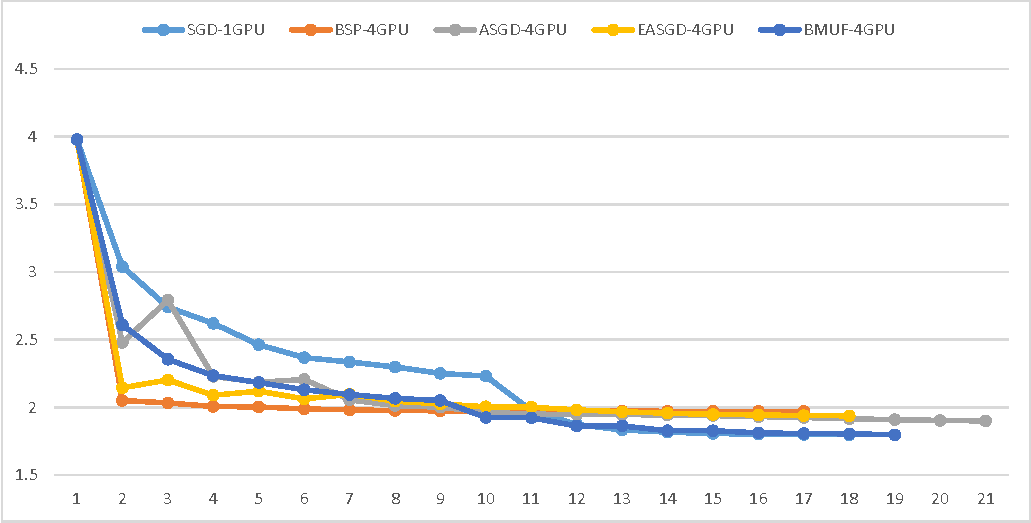
\includegraphics[width=0.8\textwidth]{figures/chapter5/dnn-crop}}
  \hspace{1in}
  \subfigure[CLDNN并行CV集上交叉熵损失]{
    \label{fig:parallel-cldnn} %% label for second subfigure
    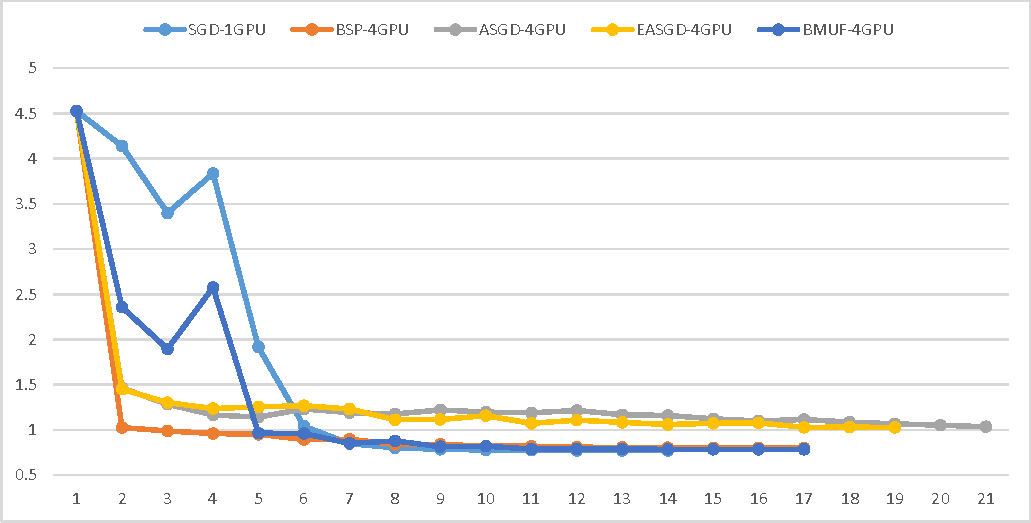
\includegraphics[width=0.8\textwidth]{figures/chapter5/cldnn-crop}}
  \caption{并行算法实验现象对比}
  \label{fig:parallel-cv} %% label for entire figure
\end{figure}

图\ref{fig:parallel-cv}中给出训练时各种并行算法随着训练轮数增加在CV集上的损失变化。如上所述,
分别给出在DNN和CLDNN两种模型上的损失变化。
可以看出,在训练初期(特别是第一轮),四种并行算法在CV集上的损失均比单卡的要低,可能是由于多卡训练时多块GPU同时处理
训练数据,训练数据的随机性更大,所以并行的模型在CV集上的损失要更好,而随着训练的进行,单卡SGD的损失则能持续平稳的下降,
并最终超过其他并行方法,BSP、ASGD和EASGD在训练后期的收敛性均不及单卡。同时也注意到,BMUF的收敛性和SGD趋势很相近,
说明BMUF算法更能接近单卡的性质。

\begin{table}[t]
\centering
\caption{aslp688 DNN并行}
\fontsize{10.5pt}{10.5pt}\song \vspace{0.5em}
\begin{tabularx}{\textwidth}{cYcYYc}
\toprule
编号 & 并行方式  & GPU数目 & CER           & 训练时间(min) & 加速比           \\ \midrule
1  & SGD   & 1     & \textbf{9.19} & 280       & —             \\
2  & BSP   & 4     & 10.09(9.79\%) & 76        & 3.68          \\
3  & ASGD  & 4     & 9.56(-4.02\%) & 75        & \textbf{3.73} \\
4  & EASGD & 4     & 9.74(-5.98\%) & 75        & \textbf{3.73} \\
5  & BMUF  & 4     & 9.24(-0.54\%) & 80        & 3.50          \\ \bottomrule
\end{tabularx}
\label{table:parallel-dnn}
\end{table}


\begin{table}[t]
\centering
\caption{aslp688 CLDNN并行}
\fontsize{10.5pt}{10.5pt}\song \vspace{0.5em}
\begin{tabularx}{\textwidth}{cYcYYc}
\toprule
编号 & 并行方式  & GPU数目 & CER           & 训练时间(min) & 加速比           \\ \midrule
1  & SGD   & 1     & \textbf{8.14} & 120       & —             \\
2  & BSP   & 4     & 8.50(-4.42\%) & 34        & 3.52          \\
3  & ASGD  & 4     & 9.01(-10.6\%) & 32        & \textbf{3.75} \\
4  & EASGD & 4     & 8.91(-9.45\%) & 33        & 3.63          \\
5  & BMUF  & 4     & 8.27(-1.59\%) & 34        & 3.52          \\ \bottomrule
\end{tabularx}
\label{table:parallel-cldnn}
\end{table}

表\ref{table:parallel-dnn}和\ref{table:parallel-cldnn}给出各种并行算法在aslp688数据集上最终的实验结果,
给出各种并行方法相对于单卡的模型精度损失(CER损失)和加速比。

分析加速比可知,四种算法在该数据集上和该硬件环境下,均能取得3.5倍以上的加速比,相差并不是很大。
主要是因为该环境为单机多卡,多卡之间的模型传输速度很快,主要时间均消耗在神经网络计算而非模型传输上,因此加速比差异并不是很大。
但同样可以看到,BSP和BMUF的加速比要比ASGD和EASGD要略差一些,因为BSP和BMUP需要所有Worker进行模型同步,
而在ASGD和EASGD中,每个Worker只需要单独和参数服务器Server进行交互,并不需要等待其他Worker。

分析模型精度可知,BMUF在DNN和CLDNN的模型上均能取得最优的并行模型精度;BSP和EASGD在两种模型上均有较大的模型损失;
ASGD在DNN上精度损失较小,但在CLDNN上模型损失较大,这与之前的实验结果和其他论文中的结果不相匹配,
因此,进行需要进行一步调优。

\subsection{ASGD调优}

实验发现,ASGD对模型的初值比较敏感。
因此使用不同轮数训练的单卡模型作为ASGD的初始模型,
图\ref{fig:asgd-init}给出了使用不同模型作为初始模型时ASGD在CV集上的收敛性。
表\ref{table:asgd-init}给出使用不同模型作为初始模型时ASGD最终的识别率实验结果。



\begin{figure}[htbp]
\centering
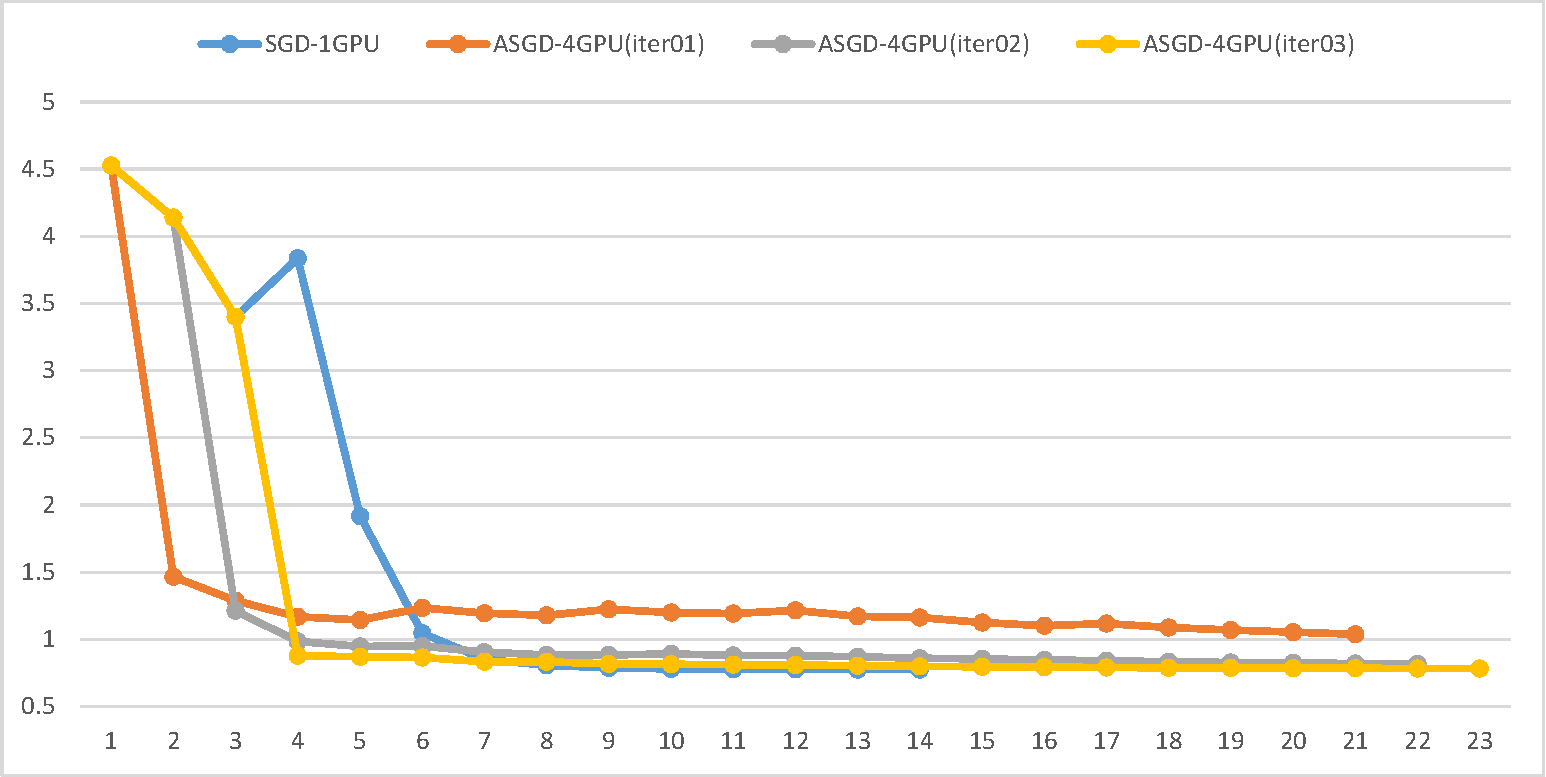
\includegraphics[width=0.8\textwidth]{figures/chapter5/asgd-init-crop}
\caption{初始模型对ASGD的影响}
\label{fig:asgd-init}
\end{figure}


\begin{table}[t]
\centering
\caption{使用不同初始模型时ASGD的最终识别率}
\fontsize{10.5pt}{10.5pt}\song \vspace{0.5em}
\begin{tabularx}{\textwidth}{cYcY}
\toprule
编号         & 并行方式                  & GPU数目      & CER                    \\ \midrule
\textbf{1} & \textbf{SGD}          & \textbf{1} & \textbf{8.14}          \\
2          & ASGD\_iter01          & 4          & 9.01(-10.6\%)          \\
3          & ASGD\_iter02          & 4          & 8.47(-3.89\%)          \\
\textbf{4} & \textbf{ASGD\_iter03} & \textbf{4} & \textbf{8.26(-1.41\%)} \\ \bottomrule
\end{tabularx}
\label{table:asgd-init}
\end{table}

其中,ASGD\_iter0x表示使用第x轮单卡训练的模型作为ASGD训练的初始模型。

可以得到,ASGD对初值模型比较敏感,使用不同的初始模型对模型的收敛性和最终效果影响很大。
使用更好的初始模型(经过更多轮数的单卡训练)时,ASGD并行训练模型的收敛性更好。
如图\ref{fig:asgd-init}所示,其在CV集上收敛性比使用较差的初始模型(经过较少的轮数的单卡训练),且CV值持续平稳下降,
并可以训练更多的轮数,最终的模型效果也要更好。

\subsection{并行训练总结}

综合以上实验结果可以得到,在该实验的四种并行方法中,BSP和EASGD模型精度损失都比较大,
因此不推荐使用这两种算法进行声学模型的并行训练。

BMUF够取得了最优的模型精度。
BMUF算法训练时的收敛趋势类似单卡SGD,具有较好的收敛性,
并最终得到更优的模型。BMUF需要Worker之间进行同步,
在各块GPU卡计算性能差别不大并且网络带宽足够的环境中,BMUF也同样可以取得不错的加速比。
Worker之间的同步也保证BMUF算法在运行多次时可以得到一致的模型。

同样ASGD也可以取得不错的模型精度,但需要更为精细的模型初始化。
ASGD中,每个Worker均只单独和Server进行通讯,无需Worker之间进行同步等待,
因此,ASGD的加速比更好,即使参与训练各块GPU卡性能不一致,也不会影响整体系统的加速性能。
ASGD Worker无需同步的潜在缺点是该系统运行多次,Worker和Server交互顺序的不一致,
可能会得到不一致的模型,不利于系统的跟踪、调试和分析。

综上,在实际使用时,应该根据实际的硬件环境和算法需求,选择合适的并行算法。

